\documentclass[a4paper,13pt]{report}
\usepackage[T1]{fontenc}
\usepackage[utf8x]{inputenc}
\usepackage[francais]{babel}
\usepackage{lmodern}
\usepackage{float}
\usepackage{graphicx}
\usepackage{amsmath}
\usepackage{amssymb}
\usepackage{listings}
\usepackage[top=2.5cm, bottom=2.5cm, left=2cm, right=2cm]{geometry}
\usepackage{fancyhdr}
\usepackage{listings}
\usepackage{url}
\lstset{
  language=C,
  basicstyle=\footnotesize,
  numberstyle=\normalsize,
}
\pagestyle{fancy}
\lhead{Chapitre \thechapter}
\rhead{Travail Personnel Encadré}
\usepackage{color}
\cfoot{\thepage}

\lstset{numbers=left, frame=single}

\title{Travail Personnel Encadré \\
Comment résoudre un problème avec un programme ?
}
\author{
  LOPEZ Aliaume \and 
  DESMARAIS Yann \and 
  SÉVIGNÉ Alfred 
  \thanks{
    Mme Sirlin | Mr Gœtz   
  }
}

\begin{document}

\maketitle
\tableofcontents

\newpage

\section*{Introduction}
  De nos jours l’utilisation de l’informatique est omniprésente… Dans de nombreux domaines scientifiques elle est utilisée comme un outil  pratique qui offre une multitude d’opportunités. Les ordinateurs sont de plus en plus performants et offrent une puissance de calcul impressionnante qui peut maintenant aider dans de nombreux domaines. Nous avons donc inscrit la problématique du TPE dans cette logique de la résolution d’un problème scientifique, et plus particulièrement biologique, grâce à un programme de simulation. Au cours de ce rapport on suivra chronologiquement l’évolution du développement de ce programme : D’abord la première partie mettra en évidence les objectifs et les buts du logiciel. Elle sera consacrée à la vision globale des fonctionnalités du programme que l’on voulait implémenter, elle constitue en quelque sorte son cahier des charges. La deuxième partie est une description du développement du programme en lui-même, elle expliquera également les expériences et recherches auxquelles nous avons procédé pour obtenir les informations nécessaires à celui-ci. Enfin la troisième partie est en premier lieu la présentation du programme final mais également une explication des limites de la simulation et des problèmes qu’il peut éventuellement soulever. \\ \\ \\


\begin{quotation}
  \textit{
    Le travail sur ce programme fut une bonne expérience, tant sur le plan virtuel que les données recherchés pour le créer. Quelques problèmes dans la création de ce programme, mais c'était l'effet recherché d'après la problématique. Le gros de nos ambitions ont pu aboutir et chacun y a mis du sien.
  }
  \begin{flushright}
    \textsc{Sévigné Alfred}
  \end{flushright}
\end{quotation}


\begin{quotation}
  \textit{
    Ce TPE a été une véritable expérience pour nous et nous a ouvert les portes de la programmation qui restait jusqu'à présent un monde assez hermétique à nos yeux.
  }
  \begin{flushright}
    \textsc{Desmarais Yann}
  \end{flushright}
\end{quotation}

\begin{quotation}
  \textit{
    Ce TPE m'a donné l'occasion de travailler avec des véritables contraintes, et un véritable but.
    Il m'a aussi permis de travailler avec des non-programmeurs ce qui m'a ouvert l'esprit quand à la réalisation d'un projet en équipe.
  }
  \begin{flushright}
    \textsc{Lopez Aliaume}
  \end{flushright}
\end{quotation}


\part{Mise en place du projet}
  \chapter{Études préliminaires}
	  \section{Objectifs}
Le but exact que nous nous sommes fixés pour le programme était l’étude du temps de vie et de division des cellules. Nous avons décidé pour plus de simplicité de nous en tenir à un seul type de cellule. Cela amena à des recherches qui nous orientèrent vers le choix des cellules de levures, qui sont des organismes eucaryotes dont le temps de division correspondait à notre échelle de temps. En effet les levures mettent deux heures pour se diviser une fois quand une cellule humaine en met vingt. Nos objectifs étaient qu’à l’aide du programme, à n’importe quel moment d’une culture de levure, on puisse savoir combien de cellules il y avait dans la colonie. Cela impliquait que le logiciel comprenne un compteur de temps et que l’on puisse stopper la simulation à tout moment pour voir l’état des cellules. A l’origine nous avions prévu deux environnements distincts dans l’interface ce qui permettait d’avoir une culture témoin et un autre test. Cette idée était motivée par le projet de soumettre aux levures des contraintes et de voir comment celle-ci y réagissait. Nous voulions en effet voir quelles étaient les différences entre une culture normale et une, par exemple, exposée à des agents mutagènes tels que les UV. Pour la représentation des cellules nous avions pensé à quelque chose de simple qui permettait une représentation sur un grand nombre de clones à l’échelle d’une colonie entière. Nous pension le menu comme une fenêtre classique avec une barre d’outil en haut ou apparaitraient les différentes fonctionnalités, les deux environnements de simulation et une barre dans le bas de la fenêtre qui afficherait les donnée de la simulation (nombres de cellules, temps de division etc). \\

\section{Recherches}

Pour réaliser cette vision première que nous avions du programme nous avons procédé il fallait réunir plusieurs conditions : 

\begin{itemize}
  \item Collecter les informations nécessaires à une simulation réaliste
  \item Faire nous même les expériences au cas où l’information n’est pas trouvée
  \item Trouver des outils informatiques performants et qui réponde à nos attentes 
  \item Trouver les fonctions impossibles à implémenter et en proposer d’autres en remplacement
\end{itemize}

Pour collecter les informations nécessaires nous avons pu utiliser internet (voir sitographie), quelque livres notamment le livre scolaire de SVT de première et de seconde (voir bibliographie), en se renseignant auprès de notre professeur de SVT voir de nos parents (les parents étaient pour chacun de nous soit biologistes soit informaticiens) pour certains détails.

Pour certaines informations concernant surtout les UV et leurs effets nous avons eu l’occasion de faire une expérience pour tester les colonies de levures exposés à ces rayonnements. Cette expérience et plus détaillée dans la partie deux dans le chapitre consacré aux UV.

Pour le choix des outils numérique nous nous sommes orientés vers un langage qui possède de nombreux avantage dont la simplicité et la rapidité. Malgré tout il avait des problèmes de portabilité. Cela nous empêcha donc de fournir le programme avec ce document, il sera présent lors de la présentation oral et sera pleinement testable…

Ensuite pour les fonctions qui n’ont pas aboutie, nous avons procédé par tâtonnement, en essayant de voir laquelle serait la plus cohérente avec l’objectif du programme et celles qui le rendrait plus pratique et facile d’accès. Nous avons par exemple ajouté le fait de pouvoir placer une grille de comptage dans chaque environnement pour mieux dénombrer les cellules, ou alors le fait de pouvoir zoomer pour voir le processus de division de plus près. 

\section{Problèmes}

Enfin il y a la question des problèmes pratiques qui interviennent dès le début du projet dans la mise en place de celui-ci. Ces problèmes étaient d’abord dans la simulation que nous voulions faire : être le plus réaliste possible en restant dans la mesure du réalisable. Trouver certaines données  a été assez difficile. Ensuite il y avait également la nécessité que le programme que nous voulions ne soit pas trop complexe à coder en définitive. En général ce ne fut pas une difficulté majeure, nous avons réussi à poser un projet réalisable et les rares fois où ce ne fut pas le cas nous nous sommes arrangés pour trouver des alternatives à ces fonctionnalités trop complexes. Enfin il y’avait les problèmes de choix personnels de chacun, nous avons dû nous mettre d’accord pour les orientations que nous souhaitions pour le logiciel. Au cours du développement et de la création du projet ce ne fut pas non plus très problématique du fait de la bonne entente du groupe et d’une communication assez régulière permettant la constatation des évolutions du programme quasiment en direct. En effet nous avions correspondances par mail importante qui se liait à l’utilisation d’une forge collaborative pour le code du programme : Github (voir sitographie).

  \chapter{Cahier des charges de la simulation}
    Avant de se lancer tête baissée dans une expérience, dans des recherches, ou dans un code, il faut impérativement avoir une idée de ce que l'on veut avoir.
Cela comprend le design, les fonctionnalités, les représentations.

Même si cette première vision est large et peut-être très éloignée du programme que nous obtiendrons au final, il faut se fixer un objectif à atteindre.

Voici un aperçu du programme : 
\begin{figure}[H]
	\begin{center}
	  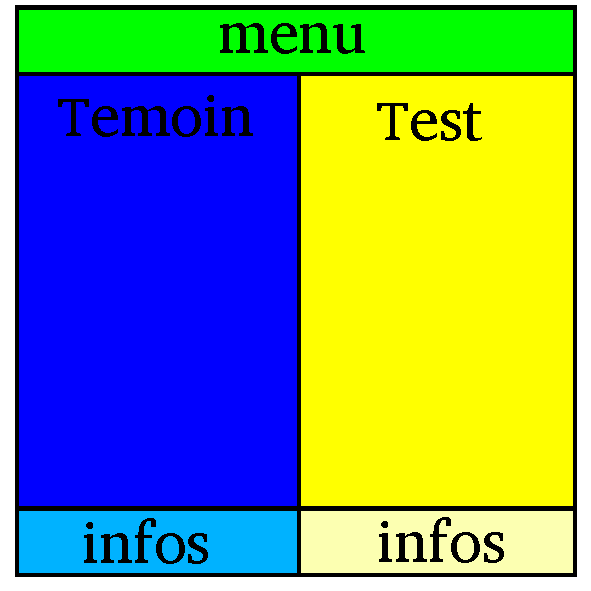
\includegraphics[width=12em]{Images/maquette.pdf}
	\end{center}
	\caption{Une première maquette}
	\label{Maquette}
\end{figure}

Nous avons : 
\begin{description}
	\item[Un menu] qui contrôle les différentes actions
	\item[Deux boites de pétri] qui représentent le témoin et le test
	\item[Une barre d'information] qui affiche les informations relatives aux simulations
\end{description}

C'est fini pour le design, maintenant il faut définir ce qu'on attend de la simulation : 
\begin{itemize}
	\item Des cellules qui se divisent
	\item Des UV qui les tuent / font muter
\end{itemize}





    
\part{Réalisation du projet}
  \chapter{Le programme}
    \section{Présentation des outils}
  Pour réaliser notre programme, il faut des outils logiciels.
  Voici une liste exhaustive des outils dont nous avons besoin, et le 
  nom ainsi que la description de ceux que nous avons choisi : 
    \begin{description}
      \item[Un ordinateur] : celui d'Aliaume 
      \item[Un langage de programmation] : nous avons choisi le Vala. Ce langage est en réalité un
        un méta-langage, un traducteur le transforme en un véritable langage de programmation : le C.
        Le C a des avantages, comme la rapidité, et des inconvénients, comme l'insécurité. Le Vala est une 
        surcouche qui permet de simplifier et de clarifier le code, en utilisant des paradigmes de programmation
        que le C n'a pas à travers une bibliothèque nommée GObject, écrite en C.
      \item[Une bibliothèque pour afficher des pixels à l'écran] : nous avons choisi la SDL, qui est une bibliothèque pour le C qui permet d'afficher des pixels à l'écran. Elle est plutôt basique, et par la même très simple. On peut donc faire tout ce que l'on veut … si l'on y met le temps de réfléchir pixel par pixels.
    \end{description}
  
  Ces choix ont été fait pour des raisons de performances, mais aussi parce que le C est un langage qui est éprouvé, et dont les vices sont tous connus. Idem pour la SDL. Tous deux sont très bien documentés. Mais, aussi parce que nous avions déjà utilisé ces outils auparavant.

\section{Programmer le contexte}
  À partir du cahier des charges de la première partie, nous savons déjà comment mettre en place tout ce qui 
  n'est pas la simulation en elle-même. Car au départ, il n'y a pas encore d'expériences, ni de résultats, on ne peut donc que réaliser ce dont on est sûr d'avoir besoin. Malheureusement, dans la plupart des cas, c'est la chose de plus complexe à réaliser.
  Par exemple, il faut créer un menu, c'est évident. Or la SDL ne propose rien de tel. Nous allons donc créer notre propre menu, de manière à pouvoir le modifier facilement au cours du développement et le réutiliser dans des programmes ultérieurs. Le menu est en fait un «~module~». L'idéal dans la programmation de nos jours, est non pas d'avoir le code avec le moins de lignes possibles, mais le code le plus lisible et le plus modulaire. Chaque module doit être indépendant des autres, être facilement modifiable et extensible.
  Voici la liste des modules qu'il faut absolument créer : 
  \begin{itemize}
    \item Le menu
    \item La boite de pétri
    \item La cellule
    \item L'affichage\footnote{Qui simplifie l'utilisation de la SDL, par exemple une fonction «~dessineCellule~» qui exécute automatiquement une liste d'instruction SDL}
  \end{itemize}
  
  Dans chaque module, il y aura différents éléments : 
    \begin{itemize}
      \item Des fonctions
      \item Des variables gobales
      \item Des Classes ou des Structures
    \end{itemize}
  Une classe ou une structure est un patron, une définition formelle d'un nouveau type.
  Après les types classiques comme les nombres ou les lettres, on a la possibilité de créer
  des combinaisons de type (on peut aussi combiner des structures). Tout ceci est définit 
  clairement dans l'annexe \ref{DefStruct} pour les structures, et \ref{DefPOO} pour les
  classes.
  
  Il faut impérativement que chaque module soit bien configurable, adaptable, réutilisable et modifiable facilement, car nous n'avons pour l'instant encore aucune idée des valeurs exactes de la simulation, il faut donc prévoir tous les cas impérativement.
  
  \begin{figure}[H]
		\centering
		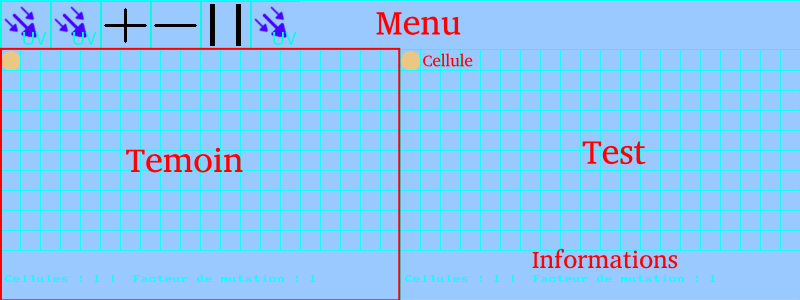
\includegraphics[width=20em]{Images/capture.png}
		\caption{Première vue du programme}
	\end{figure}


\section{Simulation et boucle principale}
  La simulation ne doit s’arrêter que quand on la quitte. On sait donc déjà qu’il y aura une boucle
presque infinie au centre du programme, afin d’éxécuter chaque action qui fait partie d’un cycle de
simulation. On peut donc imaginer une boucle principale de cette manière : 
\begin{figure}[H]
	\centering
	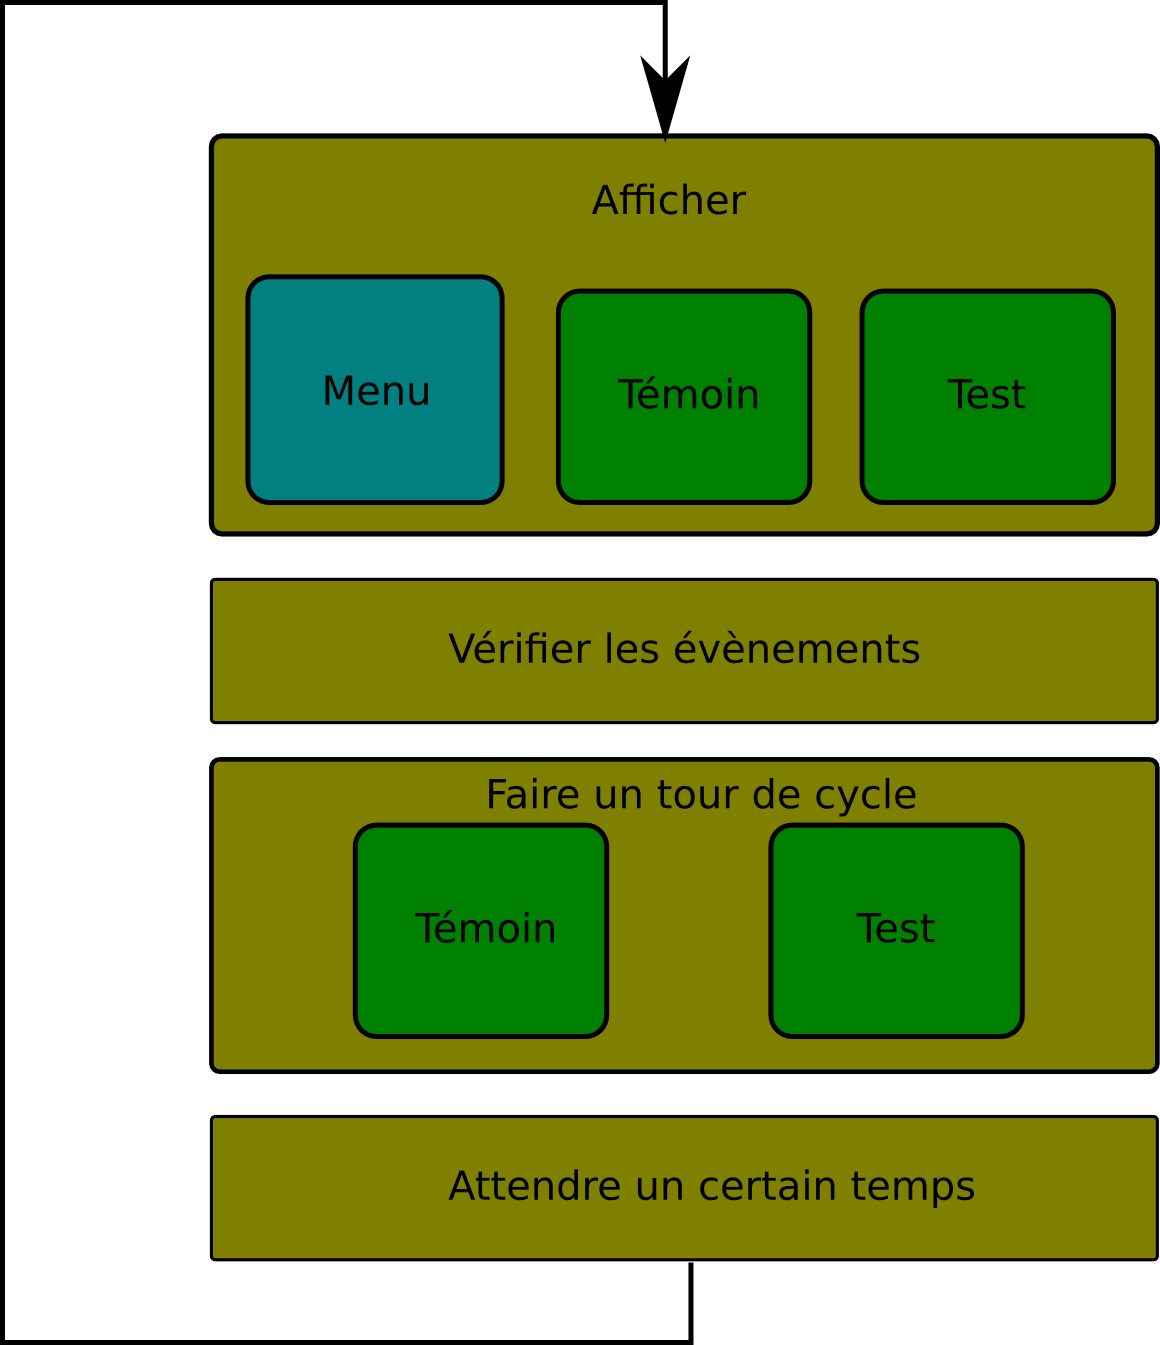
\includegraphics[width=26em]{Images/boucle_naive.png}
	\caption{Une première idée de boucle}
\end{figure}

\begin{description}
	\item[Afficher] : Dessiner le menu, la simulation témoin, la simulation test, et tout ce qu'ils contiennent sur l'écran
	\item[Vérifier les évènements] : récupérer le premier évènement produit et le traiter
	\item[Faire un tour de cycle] : exécuter\footnote{C'est un terme volontairement vague, à ce stade, on ne sait pas encore exactement ce que la simulation va faire} un tour de cycle pour la simulation témoin et la simulation test
	\item[Attendre] : Pour que la simulation soit plus constante, sans cela elle ira aussi vite que possible, et donc sera irrégulière en fonction de la densité de calcul
	\item[Recommencer] : jusqu'à ce que l'on ai demandé de quitter (géré dans les évènements)
\end{description}

On peut imaginer une vision moins naive de cette boucle en divisant les différentes actions en différents processus distincts. Cette méthode est très utile car les processus s'exécutent en parallèle ou presque\footnote{C'est le système d'exploitation qui se charge de leur répartir du temps de calcul, ils ne sont donc pas vraiment en parallèle, sauf avec les ordinateurs récents qui ont plusieurs unités de calcul (processeurs)}. Ceci permet d'avoir une 
vitesse d'affichage constante, par exemple 30 images par secondes, une vitesse d'exécution des simulation différente et une boucle qui gère les évènements avec une vitesse encore différente.

\begin{figure}[H]
	\centering
	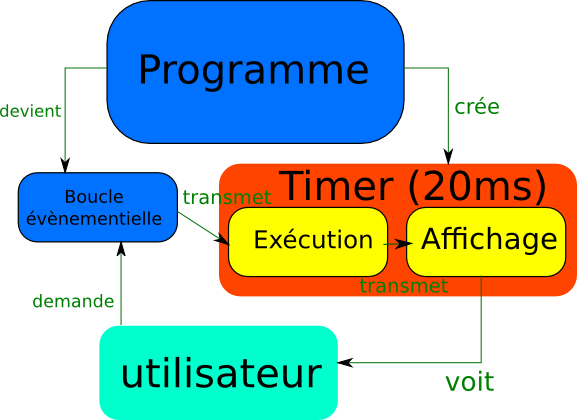
\includegraphics[width=26em]{Images/fonctionnement_programme.png}
	\caption{Fonctionnement du programme}
\end{figure}

Bien sûr il faut que les processus puissent communiquer entre eux. Et cela pose problème, étant donné qu'ils s'exécutent en parallèle, et qu'on ne sait pas lequel va être lancé en premier. On peut leur faire partager des variables, mais il faut bien vérifier qu'elle soit à jour, et éviter les modifications simultanées par deux processus d'une même variable ! C'est la seule difficulté rencontrée par la séparation en plusieurs processus, la solution a été d'utiliser des verrous : avant de faire une action on demande un verrou sur cette variable et on est sur que personne d'autre que nous ne peut la modifier, ensuite on libère le verrou, et c'est un autre processus qui prend possession de la variable. Cette méthode peut entrainer des ralentissements, des décalages, mais nous ne partageons que 2 variables, donc normalement, il n'y a pas de raisons que ces ralentissements soient visibles.


\section{Rectangle, la base}
  Nous savons que la majorité des éléments de la simulation seront affichés à l'écran.
Or pour afficher quelque chose sur une surface, il faut un certain nombre d'informations : 
\begin{itemize}
  \item Position $(x,y)$ sur l'écran
  \item Taille $(w,h)$
\end{itemize}

Nous dessinerons uniquement des rectangles, pour des raisons de simplicité, et parce que nous n'avons pas besoin d'autres formes géométriques dans notre simulation\footnote{En effet, même si on définit les cellules comme des cercles, pour afficher une image, il faut le rectangle de la taille de l'image, même si l'image elle même est un rond sur fond transparent}.

Avec ces variables, on peut ajouter plusieurs méthodes qui seront utiles :
\begin{itemize}
  \item déplacer($x$,$y$); $\rightarrow$ redéfinit la position $(x,y)$
  \item move ($x$,$y$); $\rightarrow$ effectue une translation par le vecteur $(x,y)$
\end{itemize}


Nous avons donc notre première classe : \texttt{Rectangle}, qui sera la base pour afficher des objets à l'écran.

  
\section{Le menu}
  
L'exemple du menu étant simple et parlant, nous montrerons comment nous avons pensé 
ce module. Dans un menu, il y a des boutons. Donc il faut un objet Menu\footnote{De manière à être 
utilisable dans d'autres programmes, ou pouvoir faire plusieurs menus}, et un objet Bouton. Un Bouton est un objet affiché à l'écran, il faut donc le faire hériter de Rectangle, un objet Menu a une position sur l'écran, il faut donc aussi qu'il hérite de Rectangle.

De cette manière on a maintenant des classes comme ceci :
\begin{figure}[H]
	\centering
	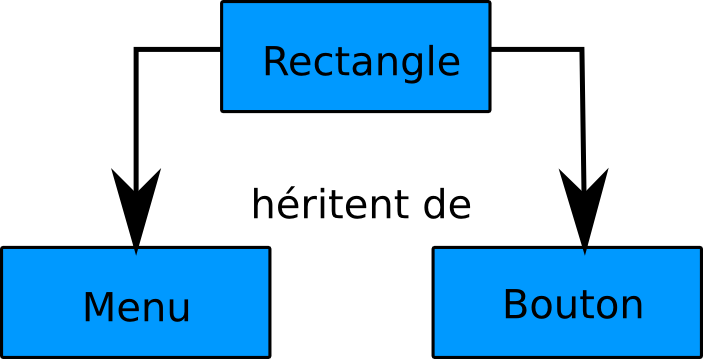
\includegraphics[width=26em]{Images/heritage_menu.png}
	\caption{Représentation de l'héritage des classes}
\end{figure} 
  
\subsection{Bouton}
	Bouton est une classe qui hérite de Rectangle, mais elle apporte son lot de nouveautés, à savoir tout ce qui est relatif au bouton : 
	\begin{itemize}
		\item une image pour le bouton normal
		\item une image pour le bouton activé
		\item une variable pour savoir si le bouton est activé
		\item une variable de type ennumération\footnote{Voir annexe \ref{DefEnum} sur les énnumération, qui parle du menu en exemple} pour savoir l'action qu'il entraine
	\end{itemize}
	
	Le bouton lui-même n'a pas vraiment de fonctions, tout le code se trouvera dans le gestionnaire des boutons, le Menu. Mais avant de parler du menu, il faut définir les actions, or nous ne savons pas encore lequelles il y aura, nous allons donc créer une énnumération, qui sera traitée dans la boucle des évènements. Ajouter une action demandera d'ajouter un item à l'énumération, et un traitement de cet item dans la boucle évènementielle.
	
\subsection{Menu}
	Le menu gère les boutons, son code n'est pas aussi complexe qu'on pourrait se l'imaginer, il contient un tableau de boutons, une fonction «~affiche~» qui affiche le menu et une fonction «~recupBouton~» qui retourne le bouton à la position du curseur.
	
	La seule difficulté réside dans le fait de dessiner correctement les boutons, et au bon endroit. Pour cela il faut savoir que l'écran de la SDL se comporte comme un repère orthonormé, à ceci près qu'il a pour origine le coin haut gauche de la fenêtre, et que son axe des Y est inversé par rapport aux graphiques habituels : 
	
	Après ça, il faut aussi savoir que le menu a une position, donc quand on place un Bouton, il faut le placer en fonction de la position du menu, et en fonction de la taille d'un Bouton. La méthode suivante est utilisée : 
	« $boutons.push(new Bouton (image,action, TAILLLE_BOUTON * numero_bouton + menu.x , menu.y,image_activé));$ ». Ce code se suffit, quand on crée un bouton, on lui donne deux images, une action, et la position du bouton vaut celle de la simulation, plus $N$ fois la largeur d'un bouton en $x$, en fonction du numéro du bouton.
	
	C'est bon, nous avons un menu fonctionnel, reste à connecter tout cela avec la boucle évènementielle et c'est terminé. Nous ne parlerons pas de la boucle évènementielle, car elle est en réalité simple. Globalement elle demande si le curseur a cliqué, si oui où. Après elle regarde sur quelle partie du programme le curseur est positionné, et un système de conditions décide de ce qu'il faut faire. Ce code n'est pas intéressant, simplement parce que c'est une suite de conditions imbriquées sans grande complexité.

    
\section{La gestion des évènements}
  \input{Parties/Ali/programme/event.tex}
\section{La gestion du temps}
  L'ordinateur ne gère pas le temps nativement. Et notre système de boucle principale non plus.
Nous savons juste qu'entre chaque cycle d'affichage il s'écoule environ 20 millisecondes, idem pour les cycles d'exécution, mais avec un «~environ~» encore plus large.
  
Il a donc fallu faire des conversions. Du fait que le programme soit configurable, il a été d'autant plus difficile de le faire, car au lieu d'ajuster les paramètres, il a fallu trouver toutes les opérations pour que les calculs fonctionnent dans tous les cas.

Par exemple quand on demande que toutes les $N$ secondes (réellement écoulées) une cellule se divise, il faut :
  \begin{itemize}
    \item $N \times 50$ pour donner des secondes (20 millisecondes entre chaque tour)
    \item À chaque tour la cellule vérifie que son nombre de tour de boucle accumulé est divisible par 
le nombre de tour de boucle nécessaire à une division : $50N$.
  \end{itemize}
  
Ceci ce complexifie quand on demande en plus que 1 seconde réelle donne $N$ minutes virtuelles.
Car tous les calculs doivent prendre en charge ce nouveau paramètre.

Il n'a d'ailleurs pas été possible de le gérer partout faute de temps, c'est pour cela que l'on gère la division des cellules en secondes réelles dans la configuration.



    
    
    
     

  \chapter{Simulation des Cellules}
		\section{Choix des cellules}
Les cellules sont la clef de voute de notre simulation, étant donné qu'elles sont les éléments principaux de celle-ci. 
La première difficulté à été de trouver quel type de cellule nous allions étudier. Pour cela nous avons effectué certaines recherches, pour trouver des cellules simples à comprendre, à manipuler et à représenter.
Cela impliquait différents facteurs : 
\begin{description}
  \item[La taille des cellules] : les bactéries sont environ 10 fois plus petites que les cellules eucaryotes 
  \item[La durée de division] : élément essentiel pour le programme, et qui varie beaucoup selon les espèces : de 20 minutes à 24h, respectivement pour les bactéries et les cellules humaines
  \item[Le métabolisme] : les éléments nutritionnels, le fait de survivre en aérobie ou non, et autre facteurs environnementaux
  \item[Le déplacement des cellules] : il existe tout types de cellules qui se déplacent ou non, et de différentes manières
  \item[L'organisation] : cellules isolées, colonies, ou organismes multi-cellulaires
\end{description}

\begin{figure}[H]
	\centering
	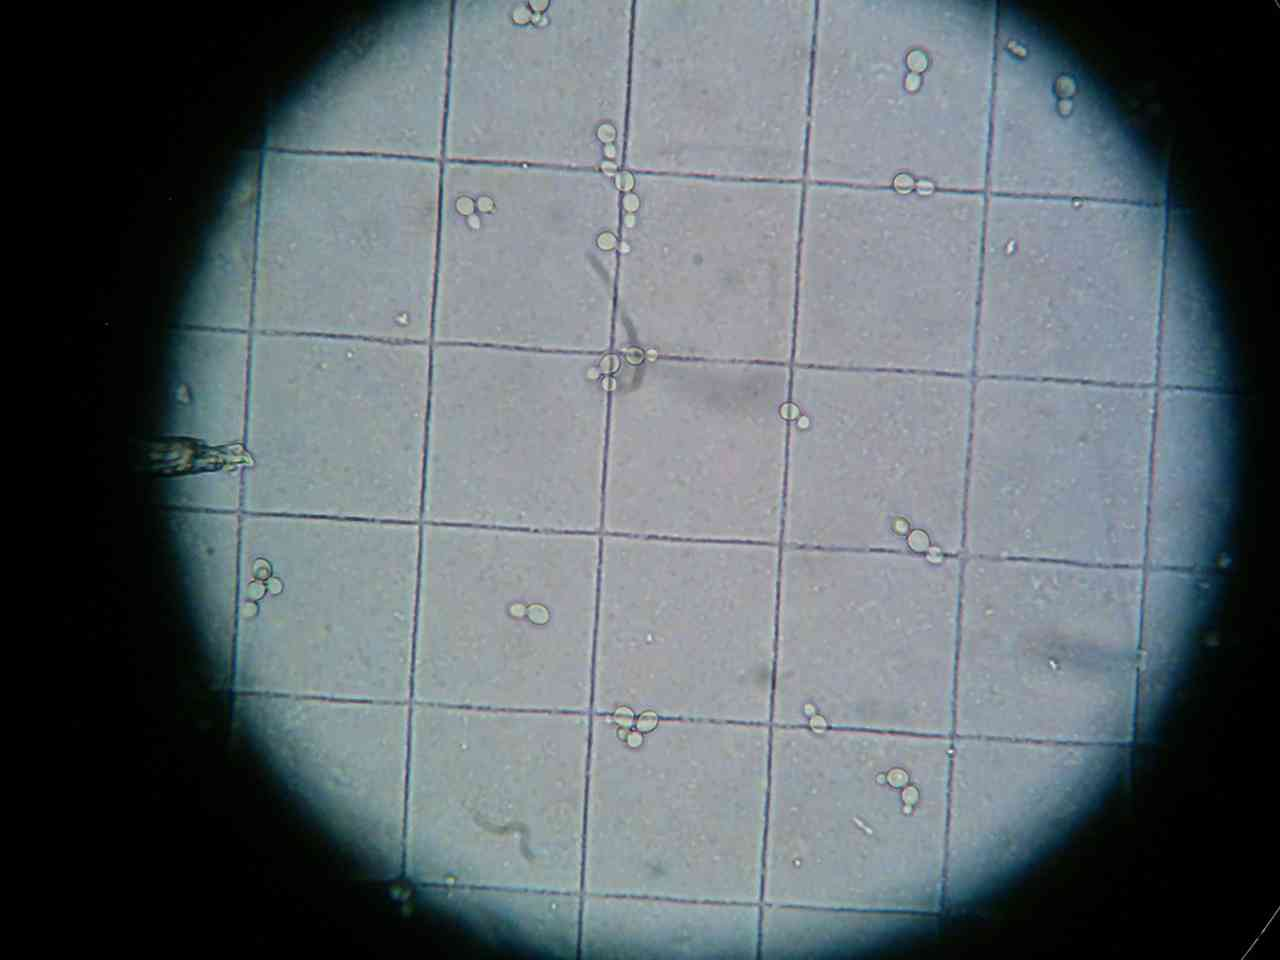
\includegraphics[width=15em]{Images/malassez.JPG}
	\caption{Cellules de Malassez}
\end{figure}

Initialement nous n'étions pas fixés sur le choix d'un type de cellule en particulier, il en découle que le programme, qui avait commencé à être développé en parallèle, peut être configuré pour certains des facteurs.

Ainsi nous avons choisi les levures, qui sont des organismes unicellulaires qui forment des colonies, qui on fait l'objet de nombreuses études précédentes. Ce qui nous a permis d'accéder facilement à des informations les concernant.
De plus les levures sont facilement mises en culture ce qui nous a permis de faire de nous en procurer facilement et de faire nos propres expériences. 

\section{Expérience personnelle}
Nous avons fait cette expérience pour avoir une idée de l'effet des UV sur les colonies de levures. 
Notre but était de soumettre les colonies à différents temps d'exposition\footnote{Mais à puissance constante}. 
Nous avions pour projet l'observation au microscope des colonies afin de dénombrer les clones mutés et le 
taux de mortalité en fonction de la durée d'exposition.
Nous voulions procéder à l'aide de lame de comptage telles que les «~cellules de Malassez~»\ref{SitoMala}.

Pour cela nous avons eu besoin de l'aide de notre professeur référent en Sciences de la Vie et de la Terre.
Ainsi à l'aide de Madame Sirlin et de X\footnote{assistante ?}, nous avons réalisé cette expérience, selon le protocole définit ci-après.

\subsection{Protocole}
  \subsubsection{Matériel}
    \begin{itemize}
      \item Six boites de pétri
      \item Des marqueurs
      \item De la levure
      \item Deux lampes à alcool
      \item Une pipette râteau
      \item De la verrerie : bécher, tube à essai …
    \end{itemize}
  \subsubsection{Étapes}
    Tout d'abord il faut créer la gélose dans laquelle nous avons ajouté du glucose, afin de constituer un environnement riche pour le développement des levures. La gélose est une substance composée d'agar-agar, sur laquelle nous allons ensemencer les souches de levure.
    
    Nous avons parallèlement produit une solution de levure de boulanger à faible concentration. 
    
    Nous avons répandu la gélose dans les boites de pétri et attendu qu'elle se solidifie. Puis, à l'aide d'une d'une pipette râteau, dans un environnement stérilisé par les lampes à alcool, nous avons répandu la solution de levure et d'eau chaude sur le milieu. 
    
    Nous avons crée 6 cultures : 
    \begin{itemize}
      \item Deux témoins qui ne seraient pas exposés aux UV
      \item Deux test qui seraient exposés aux UV durant une nuit
      \item Deux autres test qui seraient exposés aux UV durant 24h
    \end{itemize}
    
    \begin{figure}[H]
			\begin{center}
				\includegraphics[width=20em]{Images/six_levures.JPG}
				\includegraphics[width=20em]{Images/levure.JPG}
			\end{center}
			\caption{Les six boites de pétri}
		\end{figure}

\subsection{Interprétation et résultats}
  Inopportunément, nous n'avons pas eu accès à des microscopes pour analyser les résultats. De plus nous avions utilisé de la levure de boulanger, alors que pour observer des mutations visibles, il aurait fallu des levures ADE2. Malgré tout nous avons bien constaté à l'œil nu la grande disparité du nombre de colonies entre les différents test et témoins. Et donc, n'avons pu que constater la mortalité des UV, mais nous n'avons pas pu calculer des taux précis.
  Ce genre d'expérience est courante et nous avons pu trouver des résultats probants aussi bien que dans les livres de seconde et première\footnote{\ref{BibSito}}, et des expériences similaires sur internet. Ce qui nous a permis d'enchaîner facilement sur la réalisation du programme.

\subsection{Recherches complémentaires}
  Grâce à plusieurs sources nous avons obtenus les informations nécessaires au programme que nous n’avions pas pu récupérer avec l’expérience. Nos sources principales sont : le livre de première de SVT chapitre sur la génétique, activité sur l’exposition de levures aux UV et un site internet d’un professeur de SVT qui proposé le protocole et le résultat de cette même expérience\footnote{Cf \ref{BibSito}}. Dans chacun des cas nous avons pu obtenir le tableau récapitulatif des morts et mutation des levures en fonction du temps. C’est ces données que nous avons pu implémenter dans ce programme pour rendre la simulation plus ou moins réaliste lors de l’utilisation de la « fonction UV ». De plus le protocole trouvé sur internet a pu nous donner une idée de comment nous allions procéder lors de notre propre expérience. Enfin ces données ont vraiment pu compléter celles déduites de notre expérience qui, après coup, n’a pu nous fournir les informations voulues.
  
  C'est ainsi que nous avons trouvé que les levures, comme les cellules humaines, avaient un vieillissement cellulaires qui les prédéterminaient à une mort certaine environ après leur 50ème division\footnote{Cf \ref{BibSito}}
  
\subsection{Conclusion}
  À partir des informations recherchées et des interprétations que nous en avons faites, nous avons pu nous lancer dans la véritable réalisation du projet de simulation.

    \section{Choix des cellules}
Les cellules sont la clef de voute de notre simulation, étant donné qu'elles sont les éléments principaux de celle-ci. 
La première difficulté à été de trouver quel type de cellule nous allions étudier. Pour cela nous avons effectué certaines recherches, pour trouver des cellules simples à comprendre, à manipuler et à représenter.
Cela impliquait différents facteurs : 
\begin{description}
  \item[La taille des cellules] : les bactéries sont environ 10 fois plus petites que les cellules eucaryotes 
  \item[La durée de division] : élément essentiel pour le programme, et qui varie beaucoup selon les espèces : de 20 minutes à 24h, respectivement pour les bactéries et les cellules humaines
  \item[Le métabolisme] : les éléments nutritionnels, le fait de survivre en aérobie ou non, et autre facteurs environnementaux
  \item[Le déplacement des cellules] : il existe tout types de cellules qui se déplacent ou non, et de différentes manières
  \item[L'organisation] : cellules isolées, colonies, ou organismes multi-cellulaires
\end{description}

\begin{figure}[H]
	\centering
	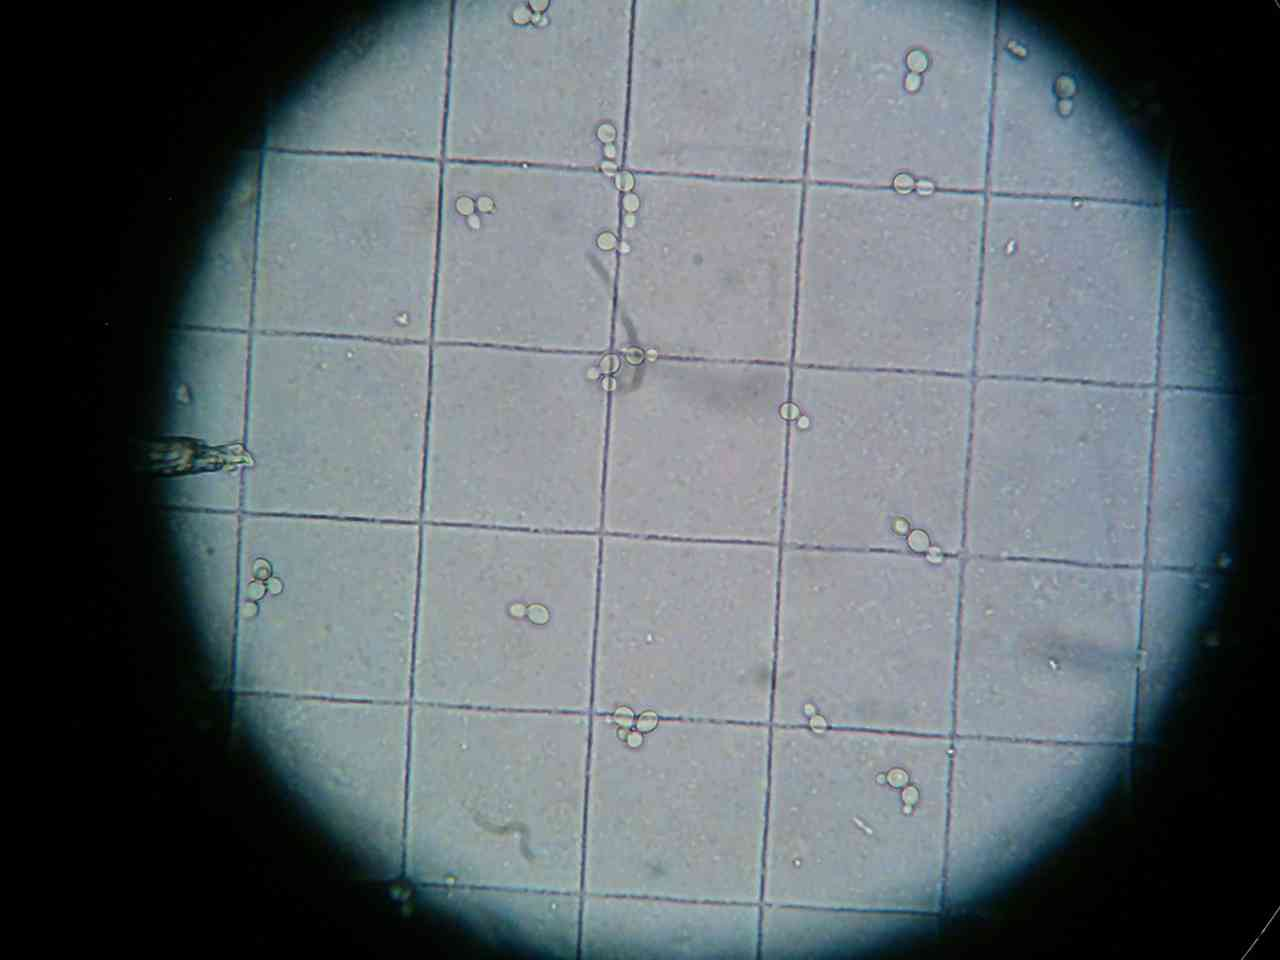
\includegraphics[width=15em]{Images/malassez.JPG}
	\caption{Cellules de Malassez}
\end{figure}

Initialement nous n'étions pas fixés sur le choix d'un type de cellule en particulier, il en découle que le programme, qui avait commencé à être développé en parallèle, peut être configuré pour certains des facteurs.

Ainsi nous avons choisi les levures, qui sont des organismes unicellulaires qui forment des colonies, qui on fait l'objet de nombreuses études précédentes. Ce qui nous a permis d'accéder facilement à des informations les concernant.
De plus les levures sont facilement mises en culture ce qui nous a permis de faire de nous en procurer facilement et de faire nos propres expériences. 

\section{Expérience personnelle}
Nous avons fait cette expérience pour avoir une idée de l'effet des UV sur les colonies de levures. 
Notre but était de soumettre les colonies à différents temps d'exposition\footnote{Mais à puissance constante}. 
Nous avions pour projet l'observation au microscope des colonies afin de dénombrer les clones mutés et le 
taux de mortalité en fonction de la durée d'exposition.
Nous voulions procéder à l'aide de lame de comptage telles que les «~cellules de Malassez~»\ref{SitoMala}.

Pour cela nous avons eu besoin de l'aide de notre professeur référent en Sciences de la Vie et de la Terre.
Ainsi à l'aide de Madame Sirlin et de X\footnote{assistante ?}, nous avons réalisé cette expérience, selon le protocole définit ci-après.

\subsection{Protocole}
  \subsubsection{Matériel}
    \begin{itemize}
      \item Six boites de pétri
      \item Des marqueurs
      \item De la levure
      \item Deux lampes à alcool
      \item Une pipette râteau
      \item De la verrerie : bécher, tube à essai …
    \end{itemize}
  \subsubsection{Étapes}
    Tout d'abord il faut créer la gélose dans laquelle nous avons ajouté du glucose, afin de constituer un environnement riche pour le développement des levures. La gélose est une substance composée d'agar-agar, sur laquelle nous allons ensemencer les souches de levure.
    
    Nous avons parallèlement produit une solution de levure de boulanger à faible concentration. 
    
    Nous avons répandu la gélose dans les boites de pétri et attendu qu'elle se solidifie. Puis, à l'aide d'une d'une pipette râteau, dans un environnement stérilisé par les lampes à alcool, nous avons répandu la solution de levure et d'eau chaude sur le milieu. 
    
    Nous avons crée 6 cultures : 
    \begin{itemize}
      \item Deux témoins qui ne seraient pas exposés aux UV
      \item Deux test qui seraient exposés aux UV durant une nuit
      \item Deux autres test qui seraient exposés aux UV durant 24h
    \end{itemize}
    
    \begin{figure}[H]
			\begin{center}
				\includegraphics[width=20em]{Images/six_levures.JPG}
				\includegraphics[width=20em]{Images/levure.JPG}
			\end{center}
			\caption{Les six boites de pétri}
		\end{figure}

\subsection{Interprétation et résultats}
  Inopportunément, nous n'avons pas eu accès à des microscopes pour analyser les résultats. De plus nous avions utilisé de la levure de boulanger, alors que pour observer des mutations visibles, il aurait fallu des levures ADE2. Malgré tout nous avons bien constaté à l'œil nu la grande disparité du nombre de colonies entre les différents test et témoins. Et donc, n'avons pu que constater la mortalité des UV, mais nous n'avons pas pu calculer des taux précis.
  Ce genre d'expérience est courante et nous avons pu trouver des résultats probants aussi bien que dans les livres de seconde et première\footnote{\ref{BibSito}}, et des expériences similaires sur internet. Ce qui nous a permis d'enchaîner facilement sur la réalisation du programme.

\subsection{Recherches complémentaires}
  Grâce à plusieurs sources nous avons obtenus les informations nécessaires au programme que nous n’avions pas pu récupérer avec l’expérience. Nos sources principales sont : le livre de première de SVT chapitre sur la génétique, activité sur l’exposition de levures aux UV et un site internet d’un professeur de SVT qui proposé le protocole et le résultat de cette même expérience\footnote{Cf \ref{BibSito}}. Dans chacun des cas nous avons pu obtenir le tableau récapitulatif des morts et mutation des levures en fonction du temps. C’est ces données que nous avons pu implémenter dans ce programme pour rendre la simulation plus ou moins réaliste lors de l’utilisation de la « fonction UV ». De plus le protocole trouvé sur internet a pu nous donner une idée de comment nous allions procéder lors de notre propre expérience. Enfin ces données ont vraiment pu compléter celles déduites de notre expérience qui, après coup, n’a pu nous fournir les informations voulues.
  
  C'est ainsi que nous avons trouvé que les levures, comme les cellules humaines, avaient un vieillissement cellulaires qui les prédéterminaient à une mort certaine environ après leur 50ème division\footnote{Cf \ref{BibSito}}
  
\subsection{Conclusion}
  À partir des informations recherchées et des interprétations que nous en avons faites, nous avons pu nous lancer dans la véritable réalisation du projet de simulation.

  \chapter{Simulation des UV}
    \input{Parties/Yann/uv.tex}
\part{Retrospective}
  \chapter{Programme final}
   
  \chapter{Limites et approfondissements}
     Le programme tel qu'il existe actuellement est fini. Mais fini ne veut pas dire qu'il est terminé.
Un programme n'est jamais terminé, il y a toujours des choses à apporter, des bugs à corriger, même les versions finales ne le sont pas. Chaque nouvelle version apporte son lot ne nouveautés, et son lot de frustration du fait de ne pas avoir pu finir tout ce que l'on voulait créer.

Le programme aujourd'hui n'est plus modifié jusqu'à la présentation orale, de manière à ne pas avoir des fonctions qui ne sont pas soigneusement décrites dans ce rapport.

Mais nous avons quand même dressé une liste des limites qu'il a actuellement, et des fonctions que l'on pourrait lui ajouter. Cette liste a été crée au fur et à mesure de la conception par toute l'équipe, chacun apportant sa vision de la simulation. Mais le plus gros des idées, viennent des personnes à qui nous avons fait tester le programme, généralement des amis ou nos parents, qui chacun dans leur domaines, ont critiqué.

\begin{description}
  \item[La forme des cellules] : les cellules sont uniquement représentées comme des rectangles de couleur. Il eu été intéressant de pouvoir mettre une image plus réaliste en conservant le jeu des couleurs. Il faudrait pouvoir définir ses propres images de cellule, ce qui permettrait de renforcer la généricité du programme.
  \item[Les caractéristiques non rendues] : le programme ne peut pas montrer de façon visible toutes les caractéristiques des cellules. Par exemple la taille de la membrane, le caryotype ou certains métabolismes. Du fait de la « surcharge » d'information que cela engendrerait. Il aurait fallu pouvoir « zoomer » sur une cellule en particulier pour avoir des informations précises sur celle-ci.
  \item[La portabilité] : le manque de portabilité du programme rend son installation sur un ordinateur plus difficile que prévue. C'est un problème non négligeable pour la distribution, il nous a par exemple été impossible de vous livrer le programme sous la forme d'un exécutable unique, du fait des librairies utilisées, qui auraient du être installées séparément, ce qui aurait été beaucoup moins simple qu'une vidéo de démonstration.
  \item[La gestion du temps] : il manque une gestion automatisée du temps qui soit plus simple et intuitive. Actuellement la configuration du programme demande une petite gymnastique mentale qui est désagréable, surtout quand on sait qu'il est possible de se l'éviter. Une autre fonctionnalité de gestion du temps serait de pouvoir modifier la vitesse de la simulation durant l'exécution du programme, pour ralentir durant l'exposition aux UV, et accélérer durant des phases de division par exemple.
  \item[Les divisions] : les divisions «~poussantes~» n'existent que pour les 4 côtés, et non pas les diagonales, il en résulte que les colonies ont une forme de losange.
  \item[La 3D] : en réalité les cellules se divisent dans l'espace tri-dimensionnel. Les levures par exemple forment des colonies sous forme de «~bulles~», qui ne dépassent pas une certaine hauteur du fait de la gravité, mais qui peut quand même être conséquente. Plutôt que de faire de la 3D, on aurait pu imaginer une légende de densité avec des couleurs, mais elle pose le problème des autres légendes qui utilisent déjà des couleurs.
  \item[L'environnement] : modifier les UV c'est bien, mais ce n'est pas vraiment suffisant, dans le principe, le logiciel devrait gérer la nutritivité de l'environnement, la température, la capacité d'ajouter des substances comme les antibiotiques. En résumer, pouvoir agir beaucoup plus sur l'environnement de la simulation.
  \item[Random] : souvent en biologie quand il faut ensemencer des cultures, on utilise des billes de verre et on secoue, ce qui a pour effet de disperser la solution de manière aléatoire et donc statistiquement quasi-uniforme. Il faudrait utiliser une fonction de ce type pour l’ensemencement de départ de la simulation.
\end{description}

\appendix
\chapter{Définition de l'Algorithmie}
  \input{Annexes/algorithmie.tex}
\chapter{Complexité algorithmique}
  \section{Definition}
  \begin{quotation}
    Quand les scientifiques se sont posé la question d'énoncer formellement et rigoureusement ce qu'est l'efficacité d'un algorithme ou son contraire sa complexité, ils se sont rendus compte que la comparaison des algorithmes entre eux était nécessaire et que les outils pour le faire à l'époque1 étaient primitifs. Dans la préhistoire de l'informatique (les années 1950), la mesure publiée, si elle existait, était souvent dépendante du processeur utilisé, des temps d'accès à la mémoire vive et de masse, du langage de programmation et du compilateur utilisé.
Une approche indépendante des facteurs matériels était donc nécessaire pour évaluer l'efficacité des algorithmes. Donald Knuth fut un des premiers à l'appliquer systématiquement dès les premiers volumes de sa série The Art of Computer Programming. 
    \begin{flushright}
      Wikipédia
    \end{flushright}
  \end{quotation}
  
  La complexité algorithmique est donc une mesure indépendante de tout facteur matériel, ou même logiciel.
  Il existe plusieures manières de calculer la complexité algorithmique, nous nous contenterons d'utiliser la plus 
  simpliste, celle qui définit l'ordre de grandeur du nombre d'opération nécessaires à la réalisation du résultat en 
  fonction nombre d'entrée N, dans le pire des cas.
  
  Par exemple le parcours d'un dictionnaire. Il y a différentes manières de coder, la méthode naïve est la suivante : parcourir tous les noms jusqu'à tomber sur le bon. Cette méthode demande au pire pour un dictionnaire de $N$ entrées un nombre $N$ d'opération (dans le pire des cas le nom est à la fin).
  Il existe aussi la méthode par dichotomie : prendre le nom du milieu. Regarder si le nom cherché est au dessus ou en dessous.
  prendre encore la moitié, et ainsi de suite. Le principe est de découper le dictionnaire en deux à chaque fois. Dans le pire des cas pour un dictionnaire de $N$ éléments, il faudra couper le dictionnaire $log_2(N)$ fois (par définition du logarithme de base deux).
  Le deuxième algorithme est donc beaucoup plus efficace que le premier. C'est là tout le principe de mesurer la complexité algorithmique de différentes méthodes, savoir les-quelles seront les plus efficaces.
    Imaginons que nous voulions accéder à la valeur $N$ d'un tableau en C : il faut effectuer une addition, puis récupérer la valeur du pointeur (cf \ref{DefTableaux}), soit une complexité de $1$.
    Mais pour accéder à la même valeur $N$ dans une liste, il faut effectuer $N$ opérations (cf \ref{DefListe}).
    
    C'est donc un bon indicateur afin de déterminer comment aborder un problème en fonction des utilisations que nous faisons des variables. 

\chapter{Archiver des données}
  En programmation il est très courant de vouloir conserver des données durant l'éxécution du programme.
Nous parlerons ici uniquement des données qui sont dans la mémoire vive, c'est à dire la mémoire tampon 
de l'ordinateur, contrairement à la mémoire morte, qui est souvent un disque dur ou un CD.
Pour conserver une information dans la mémoire vive, il faut généralement créer une variable. Nous détaillerons 
ici tout ce que l'on peut faire avec des variables.

\section{Les Types}
Une machine étant une suite de transistors, et la mémoire vive une suite de cases vides et pleines :
tout est un nombre binaire. Mais les langages de programmation permettent de faire abstraction de cette complexité techinque.
Il existe donc en Vala différents types : 
\begin{itemize}
  \item int : entier, avec des variantes commes : « uint » (entier uniquement positif), ou « int32 » (grand entier)
  \item float : nombre à virgule 
  \item double : nombre à virgule à double précision
  \item char : caractère (en réalité c'est un entier positif de maximum 256, qui est traduit en caractères ensuite)
  \item string\footnote{String = chaîne, sous entendu chaîne de caractères} : tableau de char, donc du texte vu qu'un char est un caractère.
\end{itemize}

Ces types sont la base du langage, et on les retrouve souvent car c'est la forme la plus simple de conserver une donnée.
Mais il existe un autre type, légèrement plus complexe, qui permet de faire beaucoup plus de choses.

\section{Le pointeur}
Pour commencer il faut comprendre comment fonctionne la mémoire de notre ordinateur : 
\begin{figure}[H]
  \begin{center}
	  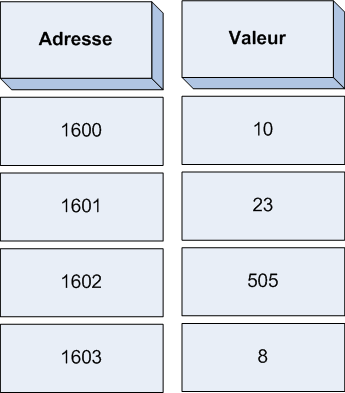
\includegraphics[width=12em]{Annexes/Images/tableau.png}
	\end{center}
	\caption{La mémoire}
\end{figure}

Ce code demande une case mémoire avec une adresse, et met le nombre 3 dedans.

\begin{lstlisting}
  int a = 3;
\end{lstlisting}

On peut récupérer l'adresse d'une variable. Par exemple pour afficher la valeur de a, puis son addresse en mémoire : 

\begin{lstlisting}
  printf ("La valeur est %d",a);
  printf ("L'adresse est %p",&a);
\end{lstlisting}

Le plus intéressant est qu'une adresse est un nombre, donc on peut la conserver dans une variable aussi !
La syntaxe est la suivante (avec type étant type du langage) : 

\begin{lstlisting}
  Type age = valeur;
  Type* pointeurSurAge = &age;
\end{lstlisting}

Ce qui donne en mémoire : 

\begin{figure}[H]
	\begin{center}
	  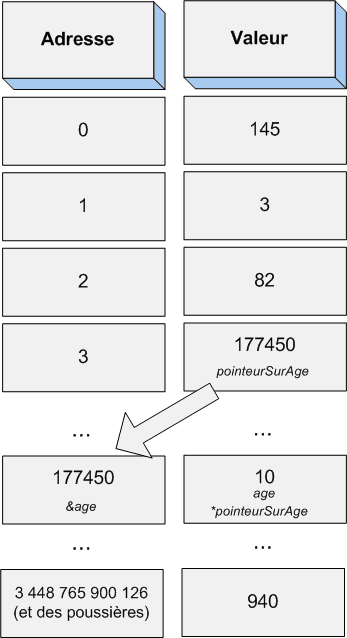
\includegraphics[width=12em]{Annexes/Images/pointeurs.png}
	\end{center}
	\caption{Un exemple de pointeur}
\end{figure}

On peut ensuite accéder à la valeure pointée par un pointeur avec la syntaxe suivante : 
\begin{lstlisting}
  *pointeurSurAge; // renvoie la valeure de age
\end{lstlisting}

Les pointeurs ne sont que des variables qui contiennent des adresses mémoire. Mais pour que l'ordinateur comprenne comment traiter la valeure pointée, le pointeur doit 
avoir le type de la variable (suivie de l'étoile du pointeur).

Une application directe du pointeur est le tableau.

\section{Tableaux}
\label{DefTableaux}
Un tableau est une suite de cases mémoire du même type : 
\begin{lstlisting}
  int tableau[4]; // Un tableau de 4 cases avec des int
  printf ("%d", tableau[1]); // valeur de la case 1
  tableau[10] = 2; // modifie une valeure du tableau
\end{lstlisting}

En réalité, voilà à quoi ressemble un tableau dans la mémoire de l'ordinateur\footnote{Image tirée de : \url{http://www.siteduzero.com/tutoriel-3-14015-les-tableaux.html}} : 
\begin{figure}[H]
	\begin{center}
	  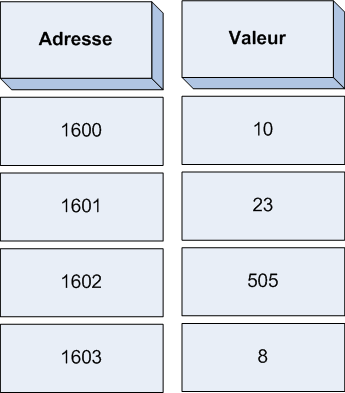
\includegraphics[width=12em]{Annexes/Images/tableau.png}
	\end{center}
	\caption{Un tableau dans la mémoire}
\end{figure}

Lorsqu'un tableau est créé, il prend un espace contigu en mémoire : les cases sont les unes à la suite des autres. L'ordinateur « saura » que c'est un tableau, et quand on demande la 3ème valeur, il prend la 3ème en partant de la première case du tableau. C'est pour cela qu'il peut y avoir les dépassements et bugs définits plus haut !

Donc en réalité, en Vala, un tableau est un pointeur vers la première variable d'une suite de variables contigues. On peut donc considérer que : 
\begin{lstlisting}
  *(tableau); // envoie la valeur de la case d'adresse 'tableau'
  tableau[0]; // envoie la case 0
  *(tableau + 3); //  envoie la valeur de la cases d'adresse 'tableau' + 3
  tableau[3]; // envoie la case 3 ( quatrieme car on compte de 0 )
\end{lstlisting}
Les syntaxes sont différentes, mais mènent au même résultat, et expliquent un peu mieux le fonctionnement du tableau.

Il en découle que le tableau a une taille fixe. Et que pour l'agrandir, il faut trouver un espace suffisant de cases mémoire contigues.

\begin{quotation}
  Le langage C n'impose pas à une implémentation de vérifier les accès, en écriture comme en lecture, hors des limites d'un tableau ; il précise explicitement qu'un tel code a un comportement indéfini, donc que n'importe quoi peut se passer. En l'occurence, ce code peut très bien marcher comme on pourrait l'attendre […] ou causer un arrêt du programme avec erreur […] ou encore corrompre une autre partie de la mémoire du processus […] ce qui peut modifier son comportement ultérieur de manière très difficile à prévoir.
  \begin{flushright}
    Wikipédia
  \end{flushright}
\end{quotation}

Il faut donc faire très attention à ne jamais dépasser la taille d'un tableau !


\section{Ennumération}
L'énnumération permet de créer un nouveau type qui peut prendre 
un certain nombre de valeurs dans un ensemble fini, imaginons un type « Volume » 
qui peut avoir uniquement les valeurs suivantes : FORT, MOYEN, FAIBLE, NULL, INFINI : 

\begin{lstlisting} 
  enum Volume {
    FORT, FAIBLE, MOYEN, NULL, INFINI
  };
  
  Volume a = Volume.FORT;
\end{lstlisting}

Ceci est utilisé pour clarifier le code, il est toujours plus lisible de faire des conditions avec des mots, plutôt qu'avec des nombres.
Par exemple, le menu a un certain nombre d'actions, au lieu de leur associer un nombre, on leur associe une valeur de l'énumération « ActionMenu ».

Mais si ceci permet quasi-uniquement de clarifier le code, il existe un moyen de créer nos propres types plus complexes.

\section{Structures}
\label{DefStruct}
Une structure est un type qui permet de combiner des variables : 
\begin{lstlisting}
  typedef struct Personne {
    int age;
    string nom;
  };
  
  Personne p;
  p.age = 16;
  p.nom = "jaques";
\end{lstlisting}

C'est à partir de cette structure que l'on peut définir des structures plus complexes.

\section{Listes}
\label{DefListe}
Les listes sont des structures plus complexes, et qui ne sont malheureusement pas gérées directement par le C ( mais par le Vala oui ).
On fait en réalité la chose suivante : 
\begin{figure}[H]
	\begin{center}
	  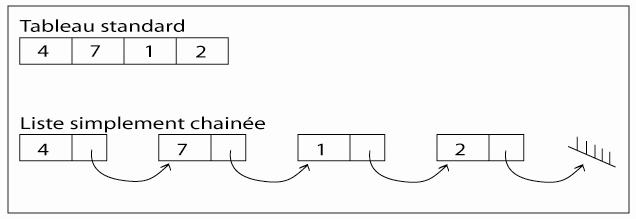
\includegraphics[width=20em]{Annexes/Images/liste.jpg}
	\end{center}
	\caption{Une liste chainée et un tableau}
\end{figure}
\begin{lstlisting}
  struct element
  {
      int val;
      element *nxt; // pointeur vers l'element suivant
  };
\end{lstlisting}

On a donc uniquement des structures qui se pointent les unes vers les autres, sans avoir besoin de zones contigues. Les opérations d'ajout et de suppression d'élément sont plus rapides : 
\begin{figure}[H]
	\begin{center}
	  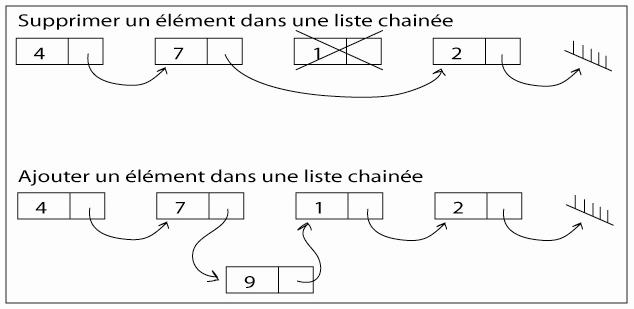
\includegraphics[width=20em]{Annexes/Images/liste_ajout.jpg}
	\end{center}
	\caption{Ajout et suppression d'un item à la liste}
\end{figure}

Mais pour récupérer un élément, on est obligé de parcourir la liste. Ce qui fait perdre du temps. Pour récupérer l'élément 3, il faut aller au un, puis au deux, et enfin regarder la valeure du numéro 3 !
Ce qui est bien moins efficace qu'un tableau. Il n'y a donc pas que des avantages, ni que des inconvénients. Les listes ne sont pas toujours simplement chainées, on peut aussi en avoir des doublement chainées, c'est à dire que chaque élément pointe vers le suivant ET le précédent. Il peut aussi y avoir des listes cycliques, c'est à dire que le dernier élément pointe vers le premier.

\chapter{Concepts avancés de programmation}
\chapter{Expériences diverses et variées}


\end{document}
